\section{Results}\label{sec:results}
\begin{equation*}
	\tfmag = 20 \times \log \left( {V_y \over V_x} \right)
\end{equation*}
\begin{equation*}
	\phi_{lag} = \phi_x - \phi_y
\end{equation*}

\subsection{Raw Measurements}

\begin{table}[htpb]
	\centering
	\begin{tabular}{@{}SSSS@{}}
		\toprule
			\textcol{$f$ (kHz)} &
			\textcol{$V_y$ (V)} &
			\textcol{$\tfmag$} &
			\textcol{$\phi_{lag}$ (\si{\degree})} \\
		\midrule
			0.5  & 0.882 & -1.065  & -22.6 \\
			1.0  & 0.708 & -2.973  & -38   \\
			2.0  & 0.46  & -6.719  & -50.4 \\
			3.0  & 0.337 & -9.421  & -53.4 \\
			4.0  & 0.267 & -11.444 & -53   \\
			5.0  & 0.224 & -12.969 & -51.1 \\
			6.0  & 0.196 & -14.129 & -48.4 \\
			7.0  & 0.178 & -14.966 & -45.6 \\
			8.0  & 0.166 & -15.572 & -43   \\
			9.0  & 0.156 & -16.111 & -41   \\
			10.0 & 0.147 & -16.628 & -38   \\
			11.0 & 0.141 & -16.990 & -36   \\
			12.0 & 0.136 & -17.303 & -33   \\
		\bottomrule
	\end{tabular}
	\caption{Response of Fig.~\ref{fig:schematic} to frequency change ($V_x = \SI{1}{\volt}$)}
	\label{table:data}
\end{table}

\subsection{Analysis}

Table~\ref{table:data} shows the response of the phase lag circuit to a range of frequencies, starting at 500\si{\hertz} then 1\si{\kilo\hertz} steps from 1\si{\kilo\hertz} to 12\si{\kilo\hertz}.
Fig.~\ref{fig:response} shows a visual representation of the magnitude and phase shift of the output over the range of 500\si{\hertz} to 12\si{\kilo\hertz}.
The measured frequency response shown in Fig.~\ref{fig:response} closely resembles the predicted, simulated response shown in Fig.~\ref{fig:response-sim}.

\begin{figure}[tbph]
	\centering
	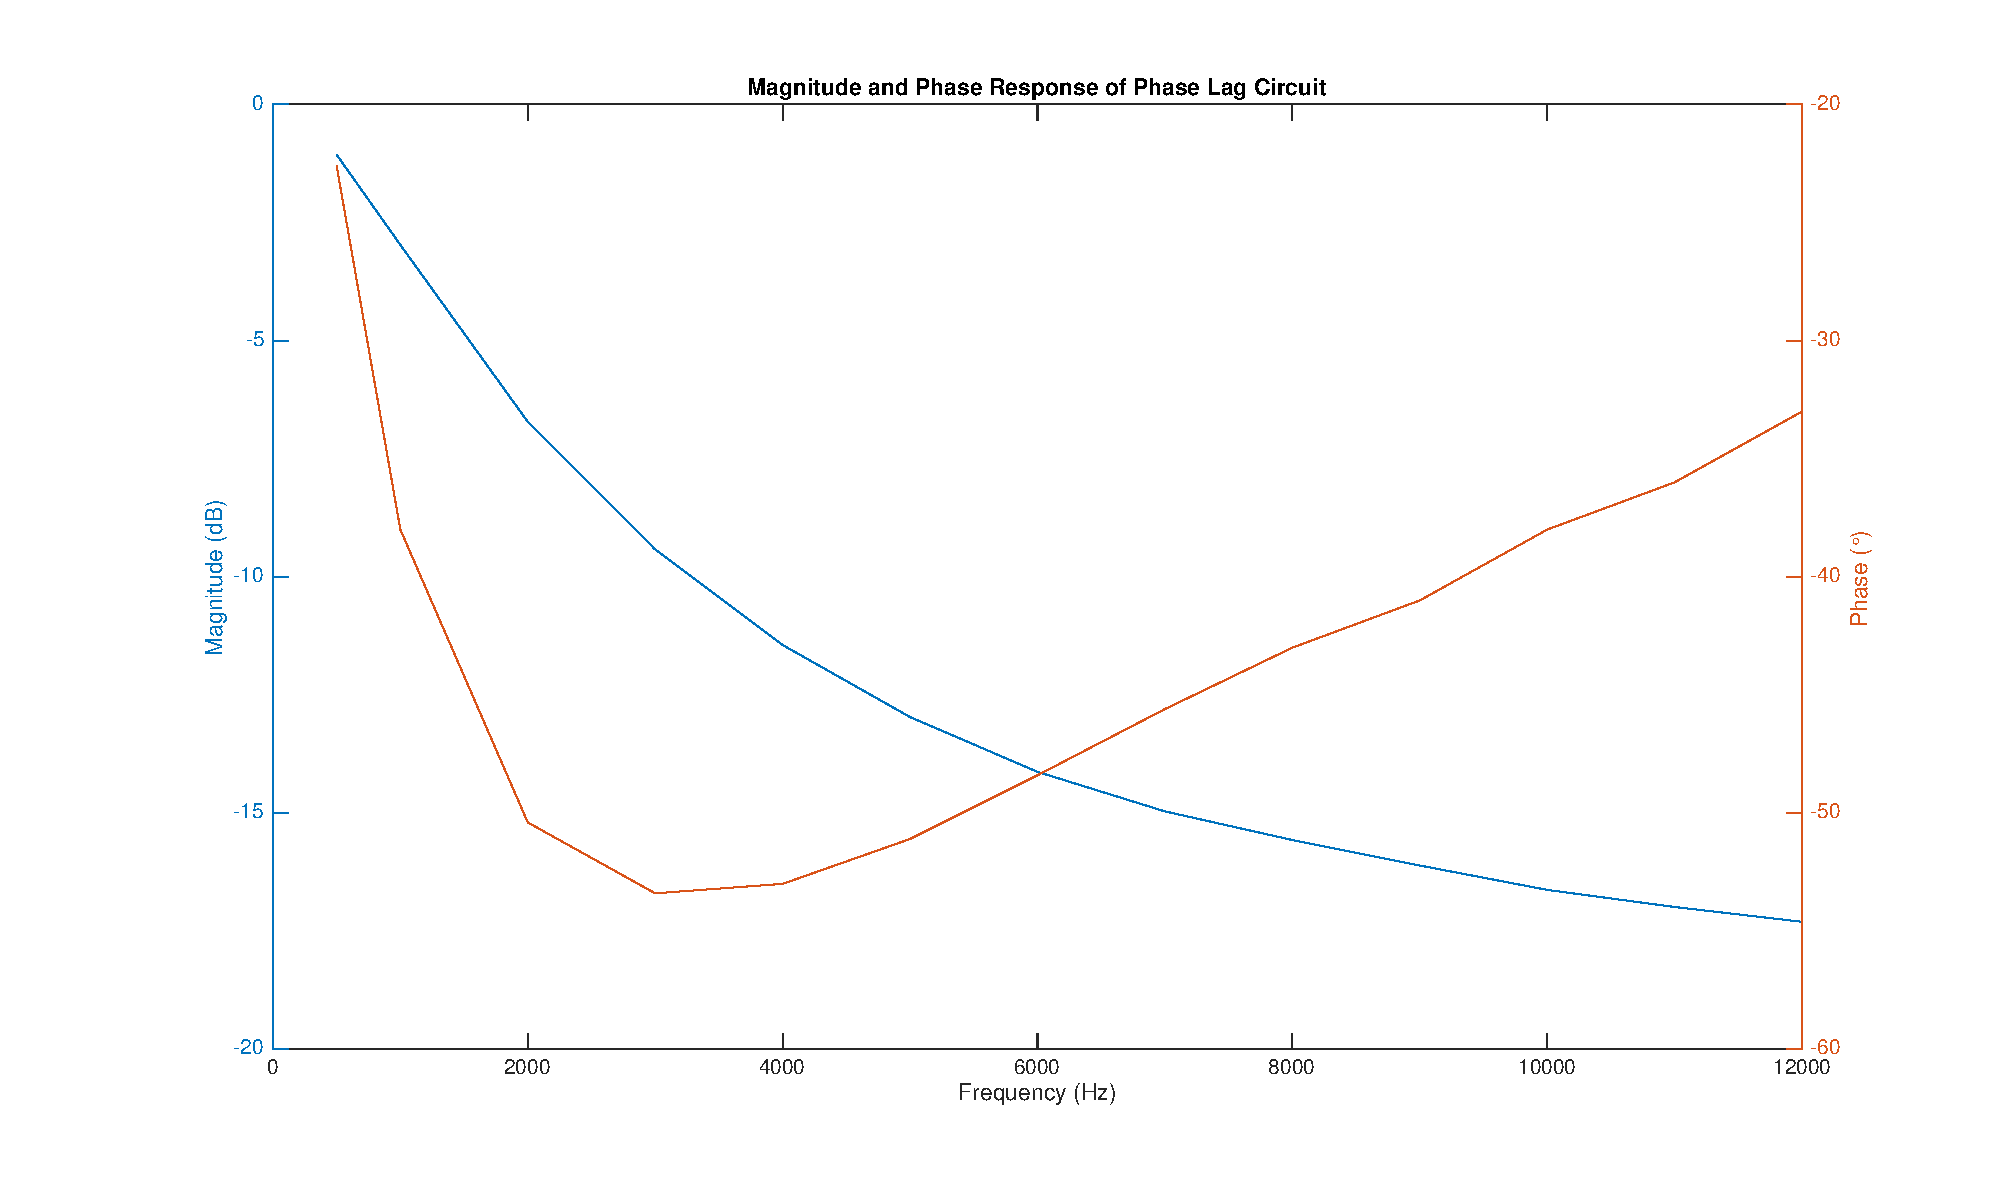
\includegraphics[width=0.8\linewidth]{graphics/response}
	\caption{Response of Fig.~\ref{fig:schematic} to frequency change ($V_x = \SI{1}{\volt}$)}
	\label{fig:response}
\end{figure}

\begin{figure}[tbph]
	\centering
	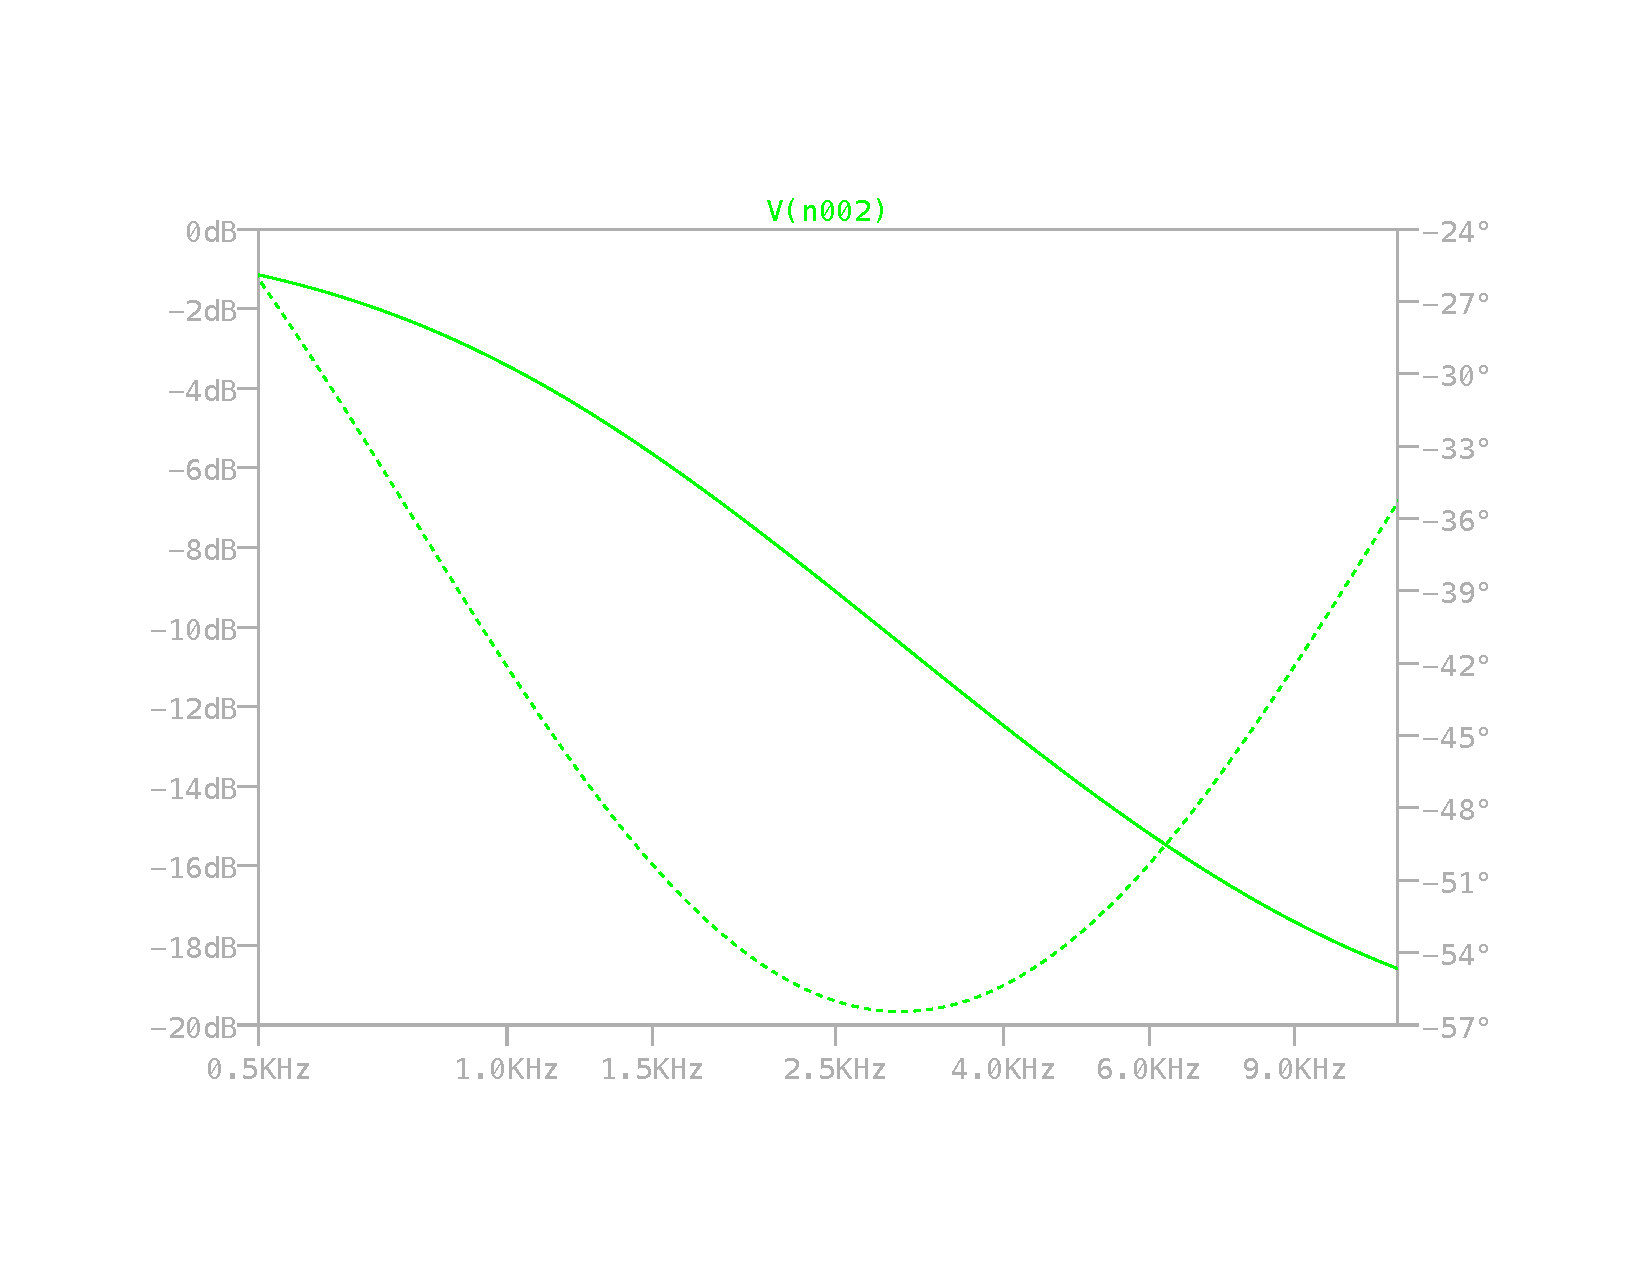
\includegraphics[width=0.8\linewidth]{graphics/response-sim}
	\caption{Simulation of Fig.~\ref{fig:schematic}'s frequency response}
	\label{fig:response-sim}
\end{figure}

The waveforms in Fig.~\ref{fig:scope}, show the phase offset of the 2 waveforms, visible by the offset in vertical cursors demonstrating a time shift.

\begin{figure}[tbph]
	\centering
	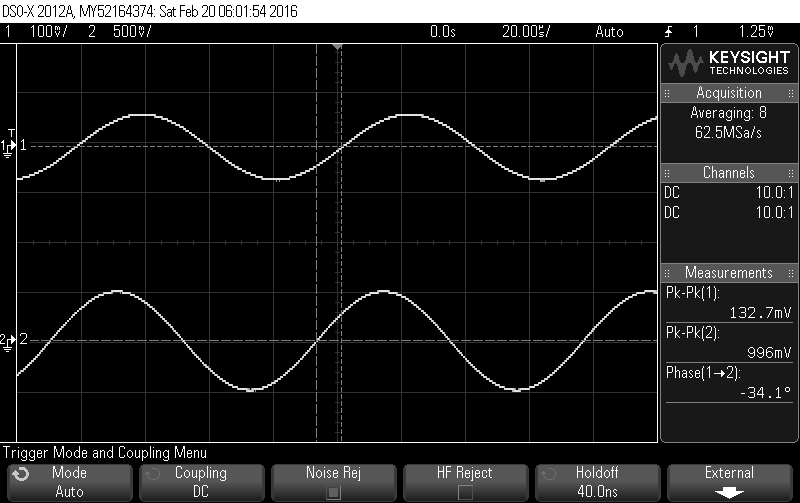
\includegraphics[width=0.65\linewidth]{graphics/12khz_phase_lag}
	\caption{$V_y(t)$ (top) lags $V_x(t)$ (bottom) by \SI{34.1}{\degree} at \SI{12}{\kilo\hertz}}
	\label{fig:scope}
\end{figure}

\clearpage
